% !TEX encoding = UTF-8 Unicode
% !TEX spellcheck = en_US

\documentclass[
	graybox,
	vecphys] % vectors bold face italic (vec command)
	{svmult}

\usepackage{makeidx} % allows index generation
\usepackage{graphicx}
\graphicspath{{./figures/}}
\usepackage{multicol}        % used for the two-column index
\usepackage[bottom]{footmisc}% places footnotes at page bottom

%%% custom commands
\newcommand{\bm}[1]{\boldsymbol{#1}}
\newcommand{\ks}[1]{{(\mathrm{CS})}_{#1}}
\newcommand{\ortvek}[4]{{ }_{(#1)}{\boldsymbol{#2}}^{#3}_{#4} }
\newcommand{\vek}[3]{\boldsymbol{#1}^{#2}_{#3}}
\newcommand{\trmat}[2]{{{ }^{#1}\boldsymbol{T}}_{#2}}
\newcommand{\rotmat}[2]{{{ }^{#1}\boldsymbol{R}}_{#2}}
\newcommand{\rotmato}[2]{{{ }^{#1}\boldsymbol{\overline{R}}}_{#2}}
% Commands for symbol of the residual (full and reduced)
\newcommand{\Res}[0]{\vec{\delta}}
\newcommand{\vecResR}[0]{\vec{\psi}}
\newcommand{\ResR}[0]{\psi}

%%% custom packages
\usepackage[T1]{fontenc}
\usepackage[utf8]{inputenc}
\usepackage{amsmath,amsfonts}
\usepackage{paralist} % for compactitem
\usepackage{siunitx}
\usepackage{url}
\usepackage{newtxtext}
\usepackage[varvw]{newtxmath} % selects Times Roman as basic font
\makeindex 

\begin{document}

\title*{Inverse Kinematics for Functional Redundancy of Symmetric 3T1R Parallel Manipulators using Tait-Bryan-Angle Kinematic Constraints}
\author{Moritz Schappler}
\institute{%
Leibniz University Hannover, Institute of Mechatronic Systems. \email{moritz.schappler@imes.uni-hannover.de}. Code: \url{github.com/SchapplM/robotics-paper_ark2022_3T1R}.}

\titlerunning{Functionally Redundant 3T1R Parallel Manipulators, Tait-Bryan-Angle Kinematics}
\authorrunning{M. Schappler}

\maketitle
\vspace{-2.5cm} % space above is reserved for author affiliations. Take the space since the one affiliation is on the footer
\abstract{% 10-15 lines long
Functional redundancy for parallel manipulators (PM) with 3T1R degrees of freedom (DoF) presents an untreated niche regarding a general and systematic kinematic description.
For an efficient formulation of the inverse kinematics problem (IKP) an existing approach using intrinsic $Z$-$Y'$-$X''$ Tait-Bryan angles for the rotational kinematic constraints is transferred from 3T3R PMs to 3T1R PMs.
The adaption of the kinematics model for the five-DoF leg chains of symmetric 3T1R PMs is elaborated in detail.
The presented application in a Newton-Raphson IK scheme with nullspace projection is validated within a dimensional synthesis of such PMs, already exploiting the redundancy.
The framework is able to reproduce existing PMs from literature.
Results show the dimensioning of PMs for an exemplary task.
}
\keywords{Parallel robot, Parallel manipulator, 3T1R, Functional redundancy, Kinematic constraints, Tait-Bryan angles, Euler angles, Dimensional synthesis.}

\section{Introduction and State of the Art}
\label{sec:introduction}

Many parallel robot structures for different degrees of freedom (DoF) of the moving platform already exist \cite{Merlet2006,KongGos2007,Gogu2008}.
%
While some few parallel manipulators (PM) are commercialized for motion with three translational DoF and fixed rotation (3T0R), such as the \emph{Delta robot}, structures for the Schoenflies motion with one rotational DoF (3T1R) are less common.
Industrially used parallel robots mainly have symmetric leg chains with motors fixed to the robot base, as this reduces costs and complexity \cite{PierrotNabComKru2009}.
One seeming example of a commercial 3T1R PM is the \emph{Adept Quattro robot}, which has four kinematic leg chains.
However, kinematically the robot is a 3T0R PM. 
The rotational DoF is transmitted via an articulated traveling plate over the fourth leg chain \cite{PierrotNabComKru2009}.
Therefore it can be classified as a parallel-hybrid structure.

The \emph{structural synthesis} of PMs with symmetric leg chains was introduced in  \cite{FangTsa2002} by using screw theory for 4-DoF and 5-DoF PMs, which results in several general rules regarding the properties of leg chains.
In \cite{HuangLi2003} screw theory is used with a constraint synthesis method for 3T1R PMs for fully-symmetrical PMs.
The \emph{Grübler-Kutzbach criterion} can be used to perform an assessment of the mobility of the synthesized lower-mobility PMs \cite{HuangLi2003,Gogu2008}, but can not provide a synthesis itself.

Extensive frameworks on the structural synthesis have been e.g. proposed by 
\cite{Gogu2008} based on \emph{evolutionary morphology} and the \emph{theory of linear transformations} and by \cite{KongGos2007} based on \emph{screw theory} and the \emph{virtual-chain} approach.
%
The results from \cite{Gogu2008} also incorporate many asymmetric PMs, e.g. of the Isoglide family, from which some have been built as prototypes.
In \cite{KongGos2007} also many symmetric PMs are proposed.
Both works give an extensive overview of possible leg chains and coupling joint alignments for parallel robots with reduced mobility, among others for 3T1R DoF.

The abundance of possible kinematic structures makes selecting the best --- or at least a suitable --- parallel robot for a 3T1R task a tedious endeavor.
Not only the kinematic structure, but also the dimensioning of kinematic parameters strongly influences performance criteria of parallel robots \cite{Merlet2006}.

A major performance criterion for parallel robots is the absence of singularities in the workspace, expressed by the condition number or other characteristics derived from the manipulator Jacobian.
A good conditioning can be accomplished by a well-chosen structural design, such as for isotropic PMs \cite{Carricato2005,Gogu2008}, where each actuator is dedicated to one platform DoF.
Another mean to avoid singularities is the use of redundant DoF.
The \emph{intrinsic redundancy} reviewed in \cite{GosselinSch2018} requires additional joints in at least one leg chain (\emph{kinematic redundancy}) or additional leg chains or actuators (\emph{actuation redundancy}).
Exploiting the \emph{functional redundancy} allows to use a DoF of the PM's operational space -- unused in the task space -- for optimization \cite{CorinaldiAngCal2016}.
%For serial-link robots this definition of task redundancy can be regarded as a sub-category of kinematic redundancy.

\emph{Optimization schemes} for functional redundancy have been investigated, such as
\begin{compactitem}
\item interval analysis in \cite{MerletPerDan2000} for a Gough platform (6-U\underline{P}S Hexapod robot\footnote{The parallel robot notation from \cite{Merlet2006} is used with prepended number of legs, chains with universal (U), revolute (R), prismatic (P) and spherical (S) joint and underlining for actuation.}), 
\item linear and quadratic programming in \cite{OenWan2007}, also for a Hexapod robot,
\item sequential quadratic programming in \cite{CorinaldiAngCal2016} for a combination of translating (3T0R) and spherical (0T3R) parallel machine,
\item the gradient-projection method on position level for general 3T3R PMs in \cite{SchapplerTapOrt2019} and on accerelation level in \cite{AgarwalNasBan2016} for a 3-\underline{R}RR and in \cite{SchapplerOrt2021} for a 6-U\underline{P}S robot.
\end{compactitem}

Several approaches exist for serial-link robots to formulate the inverse kinematics problem (IKP) properly for functional redundancy \cite{ReiterMueGat2018}.
The problem can be addressed straightforward for first- or second-order differential kinematics (on velocity or acceleration level) by using the linear Jacobian relation.
This can be transferred to parallel robots as shown for kinematic redundancy in \cite{GosselinSch2018} or explicitly for functional redundancy by \cite{AgarwalNasBan2016}.
The position-level IKP has to be handled differently due to the nonlinearity of rotation \cite{SchapplerTapOrt2019}.
%The redundant coordinate (rotation angle of the platform) is present in the common derivation of the IKP \cite{Merlet2006}.
For the \emph{explicit} IKP the substitution of the redundant coordinate is necessary for global optimization schemes, such as \cite{MerletPerDan2000}.

If only an \emph{implicit} solution of the position-level IKP is available, a numeric method such as the \emph{Newton-Raphson algorithm} can be used to obtain joint coordinates to solve the kinematic constraints equations.
This can be combined with the \emph{nullspace-projection method} and allows a local optimization of the redundant DoF while finding the IK solution.
It can also be used for kinematic redundancy, as shown by \cite{SantosSil2017} for a 3-\underline{PR}RR planar robot in combination with differential dynamic programming.
The kinematics formulation has to be handled differently than non-redundant approaches \cite{Merlet2006} to be able to exclude the redundant coordinate from the equations \cite{SchapplerTapOrt2019}.

The presented references on parallel robot redundancy mainly focus on general spatial manipulators, i.e. 3T3R PMs for 3T2R tasks \cite{MerletPerDan2000,OenWan2007,CorinaldiAngCal2016,SchapplerTapOrt2019} or planar manipulators \cite{AgarwalNasBan2016}, i.e. 2T1R PMs for 2T0R tasks.
Functional redundancy for 3T1R PMs %with spatial translation and planar rotation (3T1R DoF, Schoenflies motion) 
has not been investigated yet, to the best knowledge of the author.
A practical use for functionally redundant 3T1R PMs is not obvious, but can be motivated from axis-symmetric pick-and-place tasks, e.g. when picking parts with arbitrary rotation or with an interval of tolerance for orientation.
A technical realization of the robot end effector is e.g. a vacuum gripper with one suction cup.
Another possible application are drilling tasks in three-axis-machining or in five-axis machining using a two-DoF table orientation mechanism, similar to \cite{CorinaldiAngCal2016}.
Despite the lack of obtruding specific use cases, the sketched problem may be interesting from an academic point of view. % regarding general findings on kinematic modeling and robot synthesis.

Using functionally redundant 3T1R PMs with four leg chains instead of 3T0R PMs with three leg chains has the disadvantage of in principle smaller workspace due to additional constraints and more possible self-collisions.
Using the task redundancy for singularity and collision avoidance may on the contrary abolish these disadvantages.
This may also be beneficial for isotropic PMs of \cite{Carricato2005,Gogu2008} when nullspace optimization for collision avoidance enlarges the workspace.
In the following, an axis-symmetric 3T0R task is denoted by 3T0*R to distinguish it from fixed-orientation tasks termed with 3T0R.
In the latter case e.g. an additional revolute joint at the platform is necessary when the 3T1R PM is operated with redundant orientation.
%This parallel-hybrid machine probably is less beneficial.

The performance of the discussed alternatives can be estimated with a \emph{combined structural and dimensional synthesis}, where all possible structures are simulated for the tasks and their kinematic parameters are each optimized. %, if a custom solution is considered.
The functional redundancy has to be exploited already in the dimensional synthesis to take it's potential into account.
To be able to compare numerous different solutions, a \emph{general inverse kinematics model} is necessary.

These aspects are adressed for 3T1R PMs in this paper by adapting a kinematics model presented previously by the author based on full kinematic constraints and Tait-Bryan angles for rotation \cite{SchapplerTapOrt2019}.
%
The paper's contributions are
\begin{compactitem}
\item a novel geometric model for the IKP of task-redundant 3T1R PMs, 
\item application of the model in a gradient-projection scheme for task redundancy,
\item validation of the model in a dimensional synthesis framework.
\end{compactitem}

The remainder of the paper is structured as follows. Sect.~\ref{sec:model} presents the kinematics model which is applied in 
Sect.~\ref{sec:taskred} for the IK scheme.
The model is used in the synthesis framework, with results presented in Sect.~\ref{sec:synthesis}.
Section~\ref{sec:conclusion} concludes the paper.

\vspace{-0.3cm}
\section{Inverse Kinematic Model for 3T1R Parallel Robots}
\label{sec:model}

A fully-parallel robot with 3T1R platform mobility is considered.
The robot has $m=4$ leg chains and $n=4$ platform DoF.
It's operational-space coordinates $\vec{x}^\transp=[r_x,r_y,r_z,\varphi_z]$ contain the position $\vec{r}$ and planar orientation $\varphi_z$ of the platform-mounted end effector. % $\ortvek{0}{r}{}{D}$  and the platform rotation $\varphi_z$
Leg chains are assumed to have $n_i=5$ DoF each since six-DoF leg chains provide no constraint and four-DoF chains do not allow a symmetric PM.
%
The kinematic model is assisted by several frames, based on the model in \cite{BriotKha2015}.

Leg chains are modeled with the modified Denavit-Hartenberg parameters \cite{BriotKha2015} and the legs' kinematics can be used modularly to obtain the parallel robot kinematics.

\begin{figure}[tb]
\vspace{-0.1cm}
\input{./figures/kinematic_principle.pdf_tex}
\caption{Sketch of the kinematics model at the example of the modified 4-\underline{\`R}\`R\`R\'R\'R image of \cite{KongGos2007} (p.\,155). (\textbf{a}) All coordinate frames, (\textbf{b}) constraints for first leg chain and (\textbf{c}) other leg chains $i{\ne}1$. Joints with the same accent on \`R or \'R are parallel to each other \cite{KongGos2007}, extending the notation of \cite{Merlet2006}}
\label{fig:kinematic_principle}
\vspace{-0.2cm}
\end{figure}


The coordinate systems $\ks{}$ are sketched in Fig.~\ref{fig:kinematic_principle}a.
The world frame $\ks{W}$ serves as a reference for the relative position of task and robot, which has a base frame $\ks{0}$.
The legs are connected to the fixed base with a base joint coupling frame $\ks{A_i}$ and to the moving platform with a coupling joint frame $\ks{B_i}$.
A corresponding cut joint frame $\ks{C_i}$ is attached to the leg.
The platform has a body frame $\ks{P}$ and an additional end effector frame $\ks{E}$, which is e.g. helpful for modeling ceiling-mounted robots or additional tool transformations.
For the sake of setting up the kinematics model, the desired end effector frame $\ks{D}$ is the reference for operational space coordinate $\vec{x}$ and each leg chain has a frame $\ks{E_i}$ which corresponds to the end effector frame from the perspective of the chain $i$.
If the kinematic constraints $\vec{\Res}$ are met, i.e. $\vec{\Res}=\vec{0}$, then all $\ks{E_i}$ and $\ks{D}$ align.

The forward kinematics of each leg chain, using the leg chain's joint coordinate vector $\vec{q}_i$, is set up with $\mathrm{SE(3)}$ transformation matrices to
%
\vspace{-0.1cm}
\begin{equation}
\trmat{0}{E_i}(\vec{q}_i)=\trmat{0}{A_i} \trmat{A_i}{C_i}(\vec{q}_i)  \trmat{C_i}{B_i} \trmat{B_i}{E}.
\label{eq:fkine_leg}
\vspace{-0.1cm}
\end{equation}

The full kinematic constraints $\Res$ for all leg chains have the translational part
%
\vspace{-0.1cm}
\begin{equation}
\Res_{\mathrm{t},i}(\vec{q}_i,\vec{x})
=
\ortvek{0}{r}{}{D,E_i}(\vec{q}_i,\vec{x})
=
- \vec{x}_{\mathrm{t}} + \ortvek{0}{r}{}{E_i}(\vec{q}_i) 
\overset{!}{=}
\vec{0}
\in {\mathbb{R}}^{3}
\label{eq:phi_trans}.
\vspace{-0.1cm}
\end{equation}
%
The rotational part 
$\Res_{\mathrm{r},1}
=
\begin{bmatrix}
\alpha_{z,1} & \alpha_{y,1} & \alpha_{x,1}
\end{bmatrix}^\transp$ 
for the first leg chain $i=1$ is obtained from the rotation matrix $\rotmat{D}{E_1}$ corresponding to (\ref{eq:phi_trans}) as
%
\vspace{-0.2cm}
\begin{equation}
\Res_{\mathrm{r},1}(\vec{q}_1,\vec{x})
=
\bm{\alpha}\left(\rotmat{D}{E_1}(\vec{x},\vec{q}_1)\right)
=
\bm{\alpha}\left(\rotmat{0}{D}^\transp (\vec{x}_{\mathrm{r}})\rotmat{0}{E_1}(\vec{q}_1)\right) 
\overset{!}{=}
\vec{0}
\in {\mathbb{R}}^{3}
\label{eq:phi1_rot}
\vspace{-0.1cm}
\end{equation}
%
with the function $\bm{\alpha}(\bm{R})$, which computes the intrinsic $Z$-$Y'$-$X''$ Tait-Bryan angles $[\alpha_z,\alpha_y,\alpha_x]$ from a given rotation matrix.
Proper Euler angles like $Z$-$Y'$-$Z''$ are infeasible due to the singularity for an angle of zero.
The approach for the first leg chain is depicted in Fig.~\ref{eq:fkine_leg}b.
%
For the following leg chains, as shown in Fig.~\ref{eq:fkine_leg}c, the rotational constraints
$\Res_{\mathrm{r},i}
=
\begin{bmatrix}
\alpha_{z,i} & \alpha_{y,i} & \alpha_{x,i}
\end{bmatrix}^\transp$ 
are expressed w.r.t. the first leg chain as
%
\begin{equation}
\vspace{-0.1cm}
\Res_{\mathrm{r},i}(\vec{q}_i,\vec{q}_1)
=
\bm{\alpha}\left(\rotmat{0}{E_1}^\mathrm{T}(\vec{q}_1)\rotmat{0}{E_i}(\vec{q}_i)\right)
\overset{!}{=}
\vec{0}
\in {\mathbb{R}}^{3}
\quad \mathrm{for} \quad i=2,...,m.
\label{eq:phi2_rot}
\vspace{-0.1cm}
\end{equation}

% The translational constraints for the following leg chains are modeled in the same manner as the first leg chain in (\ref{eq:phi_trans}).
Assembling the kinematic constraints for each leg chain leads to 
%
\begin{equation}
\vspace{-0.1cm}
\Res_i^\transp=\begin{bmatrix}
\Res_{\mathrm{t},i}^\transp & \Res_{\mathrm{r},i}^\transp
\end{bmatrix} \in {\mathbb{R}}^{6}
\quad \mathrm{and} \quad
\Res^\transp
=
\begin{bmatrix}
\Res_1^\transp &
\Res_2^\transp &
\cdots &
\Res_m^\transp
\end{bmatrix} \in {\mathbb{R}}^{6m}.
\label{eq:constr}
\end{equation}
%
This formulation is designed for 3T3R PMs and is overconstraint for 3T1R PMs since six constraint equations are defined for five leg joints in the considered case.
However, it is feasible for providing a solution to the IKP. %, but does not provide a benefit regarding other approaches.
%
When considering the functionally redundant case, the reason for the selection of the rotational constraints (\ref{eq:phi1_rot}), (\ref{eq:phi2_rot}) from \cite{SchapplerTapOrt2019} becomes apparent.
The task space coordinates
$\vec{y}
=
[r_x,r_y,r_z]^\transp
$
can be obtained by removing the platform rotation $\varphi_z$.
Due to the order of rotations, the components $\alpha_{x,1}$ and $\alpha_{y,1}$ are independent of $\varphi_z$ \cite{SchapplerTapOrt2019}.
The residual $\alpha_{z,1}$ corresponds to the removed coordinate and can be disregarded.
Removing this term from the rotational constraint for the first leg chain of (\ref{eq:phi1_rot}) is termed as $\Res_{\mathrm{r},1,\mathrm{red}}$ and accordingly
%
\begin{equation}
\Res_{1,\mathrm{red}}^\transp=[\Res_{\mathrm{t},1}^\transp, \Res_{\mathrm{r},1,\mathrm{red}}^\transp] \in \mathbb{R}^5
\quad \mathrm{and} \quad
\Res_\mathrm{red}^\transp
=
\begin{bmatrix}
\Res_{1,\mathrm{red}}^\transp &
\Res_2^\transp &
\cdots &
\Res_m^\transp
\end{bmatrix} \in {\mathbb{R}}^{6m-1}.
\vspace{-0.1cm}
\label{equ:constr_red}
\end{equation}

\vspace{0.1cm} % Indices of line above go down too much
Since the leg chain has $n_1=5$ DoF and the platform has 3T1R mobility, only one DoF of the leg chain remains for the pointing direction of the $z$ axis of $\ks{E_i}$.
Therefore, for the \emph{functionally redundant case}, the \emph{translational} constraint for \emph{all} legs remains unchanged as $\vecResR_{\mathrm{t},i}:=\Res_{\mathrm{t},i}$.
For the \emph{rotational} constraint $\ResR_{\mathrm{r},1}$ of the \emph{first} leg chain (unaffected by platform rotation) a function candidate has to be found 
with
%
\vspace{-0.1cm}
\begin{equation}
	\ResR_{\mathrm{r},1}(\vec{q}_1,\vec{y})=
	\begin{cases}
		0,& \text{iff} \enspace \Res_{\mathrm{r},1,\mathrm{red}}(\vec{q}_1,\vec{y})=\vec{0} \quad \mathrm{(uniqueness~condition)} \\
		\ne 0,              & \text{otherwise.}
	\end{cases}
	\vspace{-0.1cm}
\end{equation}

The 2-norm of 
$\Res_{\mathrm{r},1,\mathrm{red}} {=} [
\alpha_{y,1}, \alpha_{x,1}
]^\transp$ 
disqualifies since the gradient w.r.t. $\vec{q}_1$ becomes 0 when approaching $\Res_{\mathrm{r},1,\mathrm{red}}{=}0$.
Instead, the constraint is selected as the 1-norm 

\vspace{-0.5cm}
\begin{equation}
\ResR_{\mathrm{r},1}(\vec{q}_1,\vec{y})
=
|\alpha_{x,1}| + |\alpha_{y,1}|
\overset{!}{=}
0
\in {\mathbb{R}}.
\label{eq:constr_rot_red_lead}
\end{equation}

The rotational constraint $\vecResR_{\mathrm{r},i}$ for the \emph{following} leg chains also contains the $z$ component $\alpha_{z,i}$, since the leading leg 1 sets the platform orientation.
Otherwise, it is constructed with the same considerations like (\ref{eq:constr_rot_red_lead}) as
%
\begin{equation}
\vecResR_{\mathrm{r},i}(\vec{q}_i,\vec{x})
=
\begin{bmatrix}
\alpha_{z,i} \\
|\alpha_{x,i}| + |\alpha_{y,i}|
\end{bmatrix} 
\overset{!}{=}
\vec{0}
\in {\mathbb{R}}^{2}
\quad \mathrm{for} \quad i=2,...,m.
\label{eq:constr_rot_red_follow}
\vspace{-0.1cm}
\end{equation}

The reduced constraints for the full robot are termed similar to (\ref{eq:constr}) as
%
\vspace{-0.1cm}
\begin{equation}
\vecResR_i^\transp=\begin{bmatrix}
\vecResR_{\mathrm{t},i}^\transp & \vecResR_{\mathrm{r},i}^\transp
\end{bmatrix} \in {\mathbb{R}}^{5}
\quad \mathrm{for} \quad i>1
\quad \mathrm{and} \quad
\vecResR^\transp
=
\begin{bmatrix}
\vecResR_1^\transp &
\vecResR_2^\transp &
\cdots &
\vecResR_m^\transp
\end{bmatrix} \in {\mathbb{R}}^{5m-1}.
\label{eq:constr_red}
\vspace{-0.1cm}
\end{equation}


The efficient computation of the 
% partial differentiation of the Tait-Bryan-angle constraints w.r.t. the joint coordinates $\vec{q}$ 
terms $\vecResR_{\partial \vec{q}}{:=}\partial  \vecResR / \partial \vec{q}$ %and the task coordinates $\vec{y}$, 
and
$\vecResR_{\partial \vec{y}}{:=}\partial \vecResR / \partial \vec{y}$,
necessary for solving the IKP,
is shown in \cite{SchapplerTapOrt2019}.
The differentiation of the absolute value of these terms can be obtained by
%
\vspace{-0.1cm}
\begin{equation}
\frac{\partial |\alpha|}{\partial \vec{q}}=\mathrm{sgn}(\alpha)\frac{\partial \alpha}{\partial \vec{q}}
\quad \mathrm{with} \quad
\mathrm{sgn}(0) \overset{!}{=} 1
\label{eq:diff_sgn}
\vspace{-0.1cm}
\end{equation}
%
to avoid a loss of differentiability.
Since the implementation is numeric, the inexactness of the signum function in (\ref{eq:diff_sgn}) does not degrade the results.

% Layout: Page should end here

%If asymmetric PMs containing leg chains $i$ with $n_i=4$ joint DoF are considered, %the component $\alpha_{x,i}| + |\alpha_{y,i}|$ has to be removed from the constraints (\ref{eq:constr_rot_red_lead}) or (\ref{eq:constr_rot_red_follow}) for that leg chain.
%the relation $\alpha_{x,i}{=}0$ and $\alpha_{y,i}{=}0$ has to hold due to the robots structure to obtain $\Res{=}\vec{0}$.
%Therefore the again reduced constraint is
%$\vecResR_1 {=} \vecResR_\mathrm{t}$ (for $i{=}1$) or $\vecResR_{\mathrm{r},i} {=} \alpha_{z,i}$ for $i{>}1$.

%components for x and y have to be constant (zero).
%Check structure via $\Res$ and not via $\vecResR$
%
%In that case, $|\alpha_{x,i}=0$ and $\alpha_{y,i}=0$ has to hold due to the robots structure.



\section{Functional Redundancy and Inverse Kinematics}
\label{sec:taskred}

The advantage of the proposed model of the previous section becomes apparent, when looking at the dimension in (\ref{eq:constr_red}) which leads for a functionally redundant symmetric 3T1R PM to a fat ``direct kinematic matrix'' \cite{Gogu2008} $\vecResR_{\partial \bm{q}}$ of dimension $19 {\times} 20$.
Using the velocity-level formulation of this matrix from the theory of linear transformations in \cite{Gogu2008} would in principle also reveal this kind of redundancy.
Approaching the formulation on the position level as shown above however is beneficial regarding the generality of the reference frame of the components corresponding to the nullspace.
The one-DoF nullspace of the matrix $\vecResR_{\partial \bm{q}}$, corresponding to  %the redundant operational space
the coordinate $\varphi_z$, can be exploited while solving the IKP.
Using the task redundancy in the overconstraint equations (\ref{equ:constr_red}) instead produces a tall $23 {\times} 20$ matrix not feasible for a numeric solution with the pseudo inverse ($\dagger$).
The inverse manipulator Jacobian $\vec{J}^{-1}$ can be obtained numerically by $\tilde{\vec{J}}^{-1}{=}{-} \Res_{\partial \bm{q}}^{\dagger} \Res_{\partial \bm{x}}$  and selecting rows corresponding to active joints. % where the overconstraint is removed numerically.

The first-order IK algorithm on position level is derived with a Taylor series expansion of (\ref{eq:constr_red}), leading to a step $k$ in the Newton-Raphson algorithm, by
%
\vspace{-0.2cm}
\begin{equation}
\vecResR(\vec{q}^{k+1},\vec{y}) =
\vecResR(\vec{q}^{k},\vec{y})
+
\vecResR_{\partial \vec{q}}(\vec{q}^k,\vec{y}) (\vec{q}^{k+1} - \vec{q}^k)
\overset{!}{=}
\vec{0}.
\vspace{-0.2cm}
\end{equation}
%
The task-related increment is obtained using the pseudo inverse as 
%
\vspace{-0.2cm}
\begin{equation}
\Delta \vec{q}^k_{\mathrm{T}}
=
(\vec{q}^{k+1} - \vec{q}^k)
=
- 
\left(\vecResR_{\partial \vec{q}}(\vec{q},\vec{y})\right)^{\dagger}
\vecResR(\vec{q}^{k},\vec{y}).
\label{equ:deltaq_psi}
\vspace{-0.2cm}
\end{equation}
%
The nullspace increment (homogeneous solution) is added, leading to
%
\vspace{-0.2cm}
\begin{equation}
{\Delta}\vec{q}
=
{\Delta}\vec{q}_{\mathrm{T}} + {\Delta}\vec{q}_{\mathrm{N}}
=
-\vecResR_{\partial\vec{q}}^{\dagger} \vecResR +  \vec{N} \bm{v}
\quad \mathrm{with} \quad
\vec{N}=\vec{I}-\vecResR_{\partial\vec{q}}^{\dagger}\vecResR_{\partial\vec{q}},
\label{equ:nullspace}
\vspace{-0.2cm}
\end{equation}
where $\bm{v}{=}h_{\partial\vec{q}}$ is the gradient of secondary tasks defined as potential $h$.
%
The formulation can also be set up on velocity level (first-order differential kinematics), based on the time differentiation of the constraints (\ref{eq:constr_red}), see e.g. \cite{Merlet2006} and similar to \cite{Gogu2008,SantosSil2017,AgarwalNasBan2016} or on acceleration level (second order) following \cite{ReiterMueGat2018,SchapplerOrt2021}.
\vspace{-0.4cm}
 %, which is omitted here for the sake of brevity.


\section{Dimensional Synthesis of Functionally Redundant 3T1R PMs}
\label{sec:synthesis}

The generality of the proposed approach for the IK model of 3T1R PMs is validated with a combined structural and dimensional synthesis.
Serial-kinematic leg chains with five joints are generated via permutation of the Denavit-Hartenberg parameters, similar to \cite{Gogu2008}. %  and isomorphism reduction
A permutation of all possible symmetric alignments of these kinematic chains is performed regarding base and platform coupling joints \cite{Gogu2008,KongGos2007,Merlet2006,BriotKha2015}, presenting the \emph{structural synthesis}.
Each combination is tested for a reference trajectory to evaluate the PM's mobility using the full model from (\ref{eq:constr}) for 3T1R task DoF.
Kinematic parameters $\bm{p}$ of the leg chains and the parallel alignment are optimized in a dimensional synthesis to obtain a feasible solution for each robot (\emph{combined synthesis}), required for the numeric evaluation in contrast to symbolic schemes.
%Computation is performed on a state-of-the-art Intel Xeon computing cluster system, using a \textsc{Matlab} implementation.


The reduced model (\ref{eq:constr_red}) is then used for a \emph{dimensional synthesis} with 3T0*R task DoF, exploiting the functional redundancy of the 3T1R PMs, as sketched in Fig.~\ref{fig:optimization_flowchart_taskred}.
The proposed kinematic model is mainly used for finding an optimal initial configuration in the position IK.
Thereby the following second-order trajectory IK starts in an equilibrium and then optimizes the same criterion, as shown in \cite{SchapplerOrt2021} in more detail.
%The IK objective criterion $h$ of (\ref{equ:nullspace}) is selected according to the objective function of the dimensional synthesis (Jacobian condition number, installation space) and the constraints that are violated in a previous iteration (e.g. self collisions, joint limits).
In this example, the kinematic objectives pursued in a Pareto optimization are Jacobian condition number, length of leg chains and installation space.
Constraints are e.g. self collisions and joint limit violations.

Examples for the resulting optimized 3T1R PMs and the trajectory are shown in Fig.~\ref{fig:results_all}a--c, proving the generality of the model by the variety of alignments.
The notation for dashes on P and R joints to mark parallelism is adapted from \cite{KongGos2007}.
The exploitation of the functional redundancy is validated with a heatmap of the performance criterion $h{=}\mathrm{cond}(\vec{J})$ over the redundant coordinate $\varphi_z$ and the trajectory progress, shown in Fig.~\ref{fig:results_all}d--e for two different robots.
The local optimization is sufficient to let the trajectory (dashed line) avoid regions of high condition numbers (dark colors) and therefore of singularities of $\vecResR_{\partial \vec{q}}$ (Type I) and of $\vec{J}$ (Type II) or of collisions and range violations (with markers according to the legend).

%The exemplary redundancy maps show that the optimal PMs for this task already give restrictions to the platform rotation.

\begin{figure}[tb]
\centering
\input{./figures/optimization_flowchart_taskred.pdf_tex}
\caption{Optimization scheme with task redundancy within the dimensional synthesis}
\label{fig:optimization_flowchart_taskred}
\end{figure}



\begin{figure}[b]
\centering
\input{./figures/robots.pdf_tex}
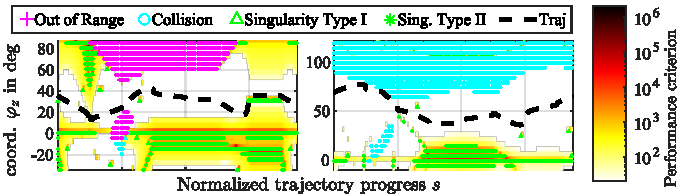
\includegraphics{perfmap_1x2.pdf}
\label{fig:results_all}
\caption{(\textbf{a}--\textbf{c}) Robots optimized for the 3T0*R task and  (\textbf{d}--\textbf{e}) two exemplary performance maps}
\end{figure}


\section{Conclusion}
\label{sec:conclusion}

%A kinematics model is presented that solves the IKP for 3T1R PMs in the presence of task redundancy.
%The generality of the approach is used in a dimensional synthesis of 3T1R PMs to obtain suitable kinematics parameters for a task-optimal PM.
%Exemplary results show the necessity of exploiting the task redundancy to find a feasible solution within the synthesis.
%The open-source framework can be used for practical application and to create variations in academic examples.

The exemplary results for the proposed IK model show the necessity of exploiting the task redundancy if a dimensional synthesis for axis-symmetric 3T0*R tasks is performed.
Optimal solutions often max out the constraints like self-collisions.
This and the problem of singularities can be diminished efficiently by nullspace optimization for reference points (on position level) and for a trajectory (on acceleration level).
The open-source framework for structural and dimensional synthesis can be used for practical application and to create variations in academic examples.

\begin{acknowledgement}
\vspace{-0.2cm}
The author acknowledges the support by the Deutsche Forschungsgemeinschaft (DFG) under grant number 341489206. \textsc{Matlab} code to reproduce the results
is available at GitHub under free license at \url{github.com/SchapplM/robotics-paper_ark2022_3T1R}.
%
\end{acknowledgement}

\vspace{-0.4cm}
\bibliographystyle{spmpsci}
\bibliography{references}

\end{document}
